%================================================================
\chapter{Introduction to Neurobiology}\label{chap:neurobio}
%================================================================

The aim of this chapter is to give a brief introduction to neurobiology, with focus on the aspects useful for understanding the biological background of the models of neural dynamics presented in the next chapter. The content of this chapter is based on material from \cite{BrainFacts}, \cite{Sterratt} and \cite{dayan_abbott}.  


%================================================================
\section{Neural Circuits and Networks}
%================================================================

The central organ of the human nervous system is the brain, which contains roughly 86 billion nerve cells, or neurons, organized in different brain regions specialized at analyzing different subsets of information encoded in nerve signals. Brain activity is made possible by the interconnections of neurons. A population of neurons interconnected to carry out a specific function is called a \textit{neural circuit}. Neural circuits interconnect to one another to form elaborate \textit{neural networks} that route signals through the different regions of the brain, analyzing and organizing different types of information within fractions of a second. Neurons are either \textit{excitatory} or \textit{inhibitory}. Excitatory neurons are predominant, comprising about 80\% of the neurons in the brain, and send signals to neighboring neurons that increase activity. By contrast, inhibitory neurons, comprising about 20\% of the neurons in the brain, send signals that suppress the activity of neighboring neurons. Every neural circuit contains both excitatory and inhibitory neurons that work together to regulate the actitivy in response to stimuli. 

%================================================================
\section{Neurons}
%================================================================

The fundamental unit of neural circuits and networks is the neuron, which is a specialized cell that generates electrical signals in response to stimuli and transmits them to other cells. Although neurons come in a wide variety of shapes and sizes, they have common morphological specializations called \textit{dendrites} and \textit{axon}. Like other cells, a neuron consists of a cell body (soma) that contains the neuron's nucleus and molecular machinery critical to the cell's function, and the soma is confined by a cell membrane that consists of a lipid bilayer. The axon and dendrites are filaments that extrude from the soma, as illustrated by \autoref{fig:neuron_morph}. Dendrites receive incoming signals from other neurons and propagate them to the soma. The branching structure of the dendritic tree allows a neuron to receive signals from many other neurons. The soma processes the collected input signals and generates an output signal if the total input exceeds a certain threshold. The axon carries the output signal and branch out to deliver the signal to other cells through the axon terminals. 


\begin{figure}[!htb]
    \centering
    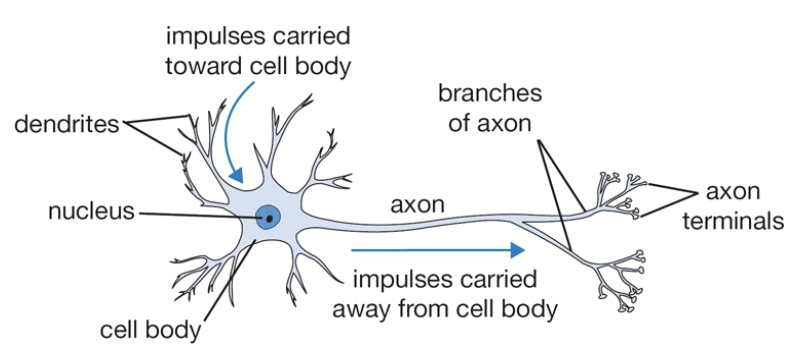
\includegraphics[scale=0.7]{neuron_morph}
    \caption{Schematic illustration of a neuron. A neuron can be divided into three functionally distinct parts called dendrites, the cell body (soma) and the axon. The dendrites receive signals from other neurons and transmit them to the cell body, which can generate an output signal if the total input exceeds a threshold. The output signal propagates down the axon which branch out and end in axon terminals that deliver the signal to other cells.
    }
    \label{fig:neuron_morph}
    \source{\cite{neuron_morph}.}
\end{figure}


%================================================================
\section{Ion Channels and Action Potentials}\label{sec:ion_ch_and_ap}
%================================================================

The bulk of the neuronal membrane is composed of a \textit{lipid bilayer}, that is made up of two layers of lipids, which have their hydrophilic heads pointing outwards and their hydrophobic tails pointing inwards. It is virtually impermeable to water molecules and ions. \textit{Ion channels} are protein pores in the neuronal membrane that allow ions, predominantly sodium (\Na), potassium (\K), calcium (Ca$^{2+}$) and chloride (Cl$^{-}$), to flow into and out of the neuron. Most ion channels are permeable only to specific types of ions, and are either active or passive. Passive channels, also called leakage channels, are always permeable, whereas active channels have gates that can open and close the channel. Some active ion channels are voltage-gated, meaning that whether the channel is in an open or closed state is controlled by voltage, while others are chemically-gated, meaning they open and close by interactions with chemicals. The neuronal membrane also contains membrane-spanning protein structures that actively pump certain types of ions into and out of the neuron, called \textit{ion pumps}. Ions tend to flow from regions of high concentration toward regions of low concentration, thus diminishing the concentration gradient. Ion pumps counteract this by pumping ions against the concentration gradient. For instance, the \Na -- \K pump exchanges three \Na from inside the cell with two \K from outside using energy provided by hydrolysis of ATP into ADP and a phosphate ion. \autoref{fig:neuronal_membrane} illustrates the constituents of the neuronal membrane. 

\begin{figure}[!htb]
    \centering
    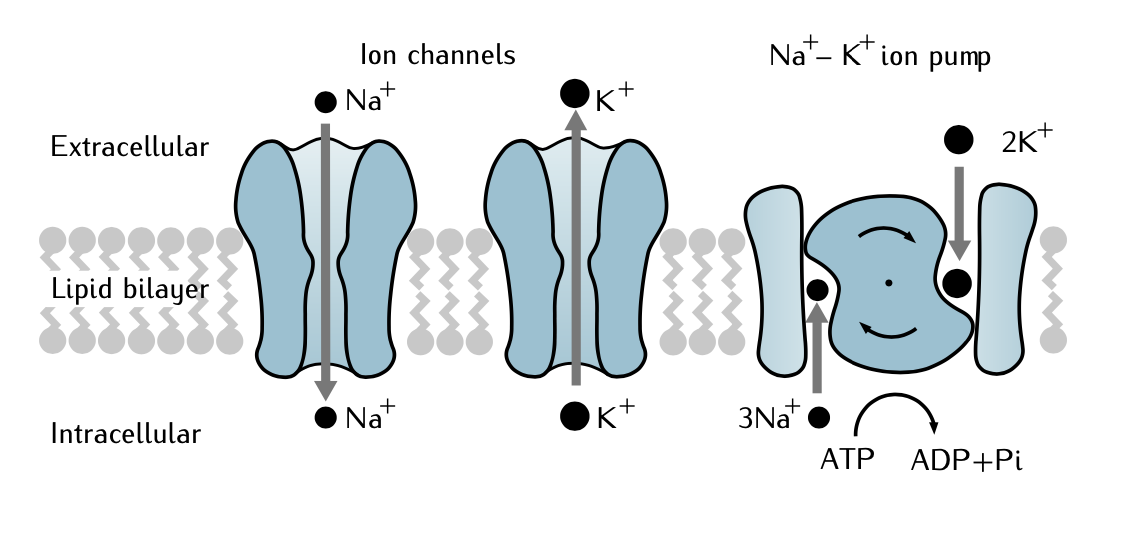
\includegraphics[scale=0.6]{neuronal_membrane}
    \caption{Constituents of the neuronal membrane. The lipid bilayer forms a virtually impermeable barrier for inorganic ions. Ion channels form pores in the neuronal membrane, allowing certain ions to flow into and out of the neuron. Ion pumps exchange certain ions across the neuronal membrane. 
    }
    \label{fig:neuronal_membrane}
    \source{\cite{Sterratt}.}
\end{figure}

Due to the ion channel and pump machinery, there is typically a greater concentration of \Na in the extracellular space and \K inside the neuron. Moreover, there are slightly more positive ions on the outside of the neuron and slightly more negative ions on the inside. Hence, there is a small electrical potential difference across the neuronal membrane, called \textit{membrane potential}. The membrane potential of a resting neuron, known as the \textit{resting membrane potential}, typically lies between $-60$ and $-70 \mV$, because the potential is more negative inside the neuron than on its outer surface. The membrane potential is affected by signals received from other neurons in its circuit, which can make the membrane potential less negative (depolarized) or more negative (hyperpolarized). If a neuron is depolarized sufficiently to raise the membrane potential above the membrane's threshold voltage, a positive feedback process is initiated which triggers an electrical impulse called an \textit{action potential} (AP). The temporal evolution of APs can be divided into different phases, as shown by \autoref{fig:action_potential}.
\begin{figure}[!htb]
    \centering
    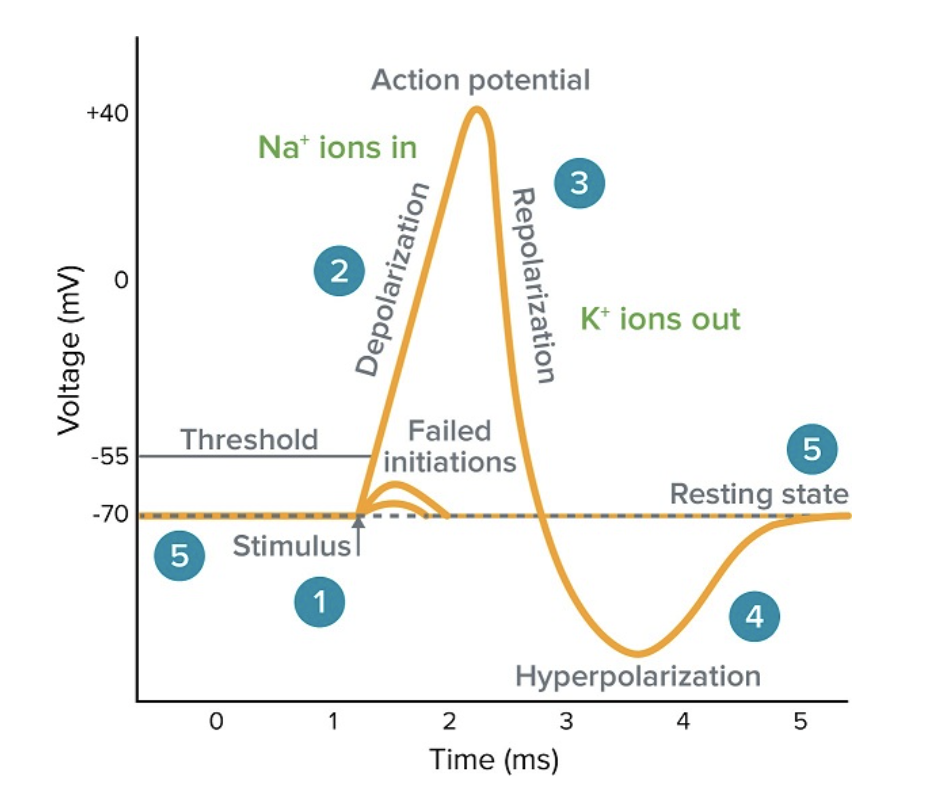
\includegraphics[scale=0.6]{action_potential}
    \caption{The temporal evolution of the membrane potential during a typical action potential. The membrane potential is initially in its resting state when (1) a stimulus pushes it over the threshold. (2) This results in a rapid rise (depolarization) in membrane potential caused by opening of voltage-gated sodium (\Na) channels that give in an influx of \Na ions. (3) This is followed by a sharp decrease (repolarization) in membrane potential caused by closing of sodium channels and opening of potassium (\K) channels that give an efflux of \K ions. (4) The membrane potential typically undershoots the resting potential (hyperpolarization) before it gradually recovers to the (5) resting state. 
    }
    \label{fig:action_potential}
    \source{\cite{action_potential}.}
\end{figure}
First, stimulus from other neurons connecting to the neuron depolarizes the soma, and increase the membrane potential towards the threshold potential. If the threshold potential is reached, voltage-gated sodium channels open and an influx of sodium ions takes place. This phase is called \textit{depolarization}. During depolarization, the inside of the neuron becomes increasingly electropositive. Once the membrane potential becomes positive, the membrane potential continues to depolarize, commonly referred to as AP \textit{overshoot}, until it reaches the electrochemical equilibrium, known as the \textit{reversal potential}, and peaks. After the overshoot, sodium channels decrease the sodium permeability by closing. The overshoot also opens voltage-gated potassium channels, which cause a potassium efflux that decreases the neuron's electropositivity. This phase is called \textit{repolarization}, and decreases the membrane potential towards the resting state. Repolarization may be followed by \textit{hyperpolarization}, in which the neuron's membrane potential falls below the resting potential before gradually recovering to the resting potential. The hyperpolarizing phase where the membrane falls below the resting potential is commonly referred to as \textit{afterhyperpolarization} (AHP) or AP \textit{undershoot}.  

The resulting AP will propagate along the axon towards the next neurons in the circuit. APs are also known as \textit{spikes}, and a temporal sequence of APs generated by a neuron is called a \textit{spike train}. A neuron that emits an AP is often said to \textit{fire}, and the frequency a neuron emits APs is therefore called the \textit{firing rate} of the neuron. Generation of APs depends on the recent history of the neuron firing. In the brief \textit{absolute refractory period} after an AP, it is virtually impossible to initiate another AP, regardless of the amplitude of the stimulus. For a longer interval known as the \textit{relative refractory period}, the threshold for firing is higher than when the membrane is at rest, and APs initiated in this period have lower peak voltage. 


%================================================================
\section{Synapses}
%================================================================

APs are passed from a neuron to next at junctions called \textit{synapses}, which are usually formed between axon terminals on the sending neuron and the dendrites of the receiving neuron, with a space between the two called the \textit{synaptic cleft}. It is common to refer to the sending neuron as the \textit{presynaptic} neuron and the receiving as the \textit{postsynaptic} neuron. The cleft of most synapses is too wide for APs to directly impact the postsynaptic neuron. Instead, chemical signals called \textit{neurotransmitters} cross the synapse. Excitatory neurons release neurotransmitters to increase the activity of the postsynaptic neuron, making it more likely to generate an AP,  while inhibitory neurons release neurotransmitters to suppress the activity, making the postsynaptic neuron less likely to generate an AP.
